\documentclass[t]{beamer} % add 'handout' to remove animations, add t to remove centering
\usepackage[utf8]{inputenc}
 
\usetheme{Boadilla} % the nicest theme imho 

\usepackage{parskip} % adds space between paragraphs
 
%Information to be included in the title page:
\title[Intermediate {\LaTeX} Topics]{Intermediate {\LaTeX} Topics in Action}
\subtitle{A Wonderful Presentation}

\author[D. Z. Garza, D. O. Henriksson]{Zack Garza and Oskar Henriksson}
\institute[UCSD]{University of California, San Diego}
\date{\today}
 
 
\begin{document}
 
\begin{frame}
\titlepage
\end{frame}

\begin{frame}[fragile]{Outline} %fragile is necessary to make \verb work

    In this presentation, we will prove a historically important result from number theory (yep, you guessed it: it's the irrationality of $\sqrt{2}$) and at the same time showcase some of the basic features of Beamer such as the \verb$frame$ and \verb$itemize$ environments and the $\visible<>$ command.
    
    In the next slide, we use \verb$\tableofcontents$ to show the structure of the presentation. We use the command \verb$\section$ in the rest of our document to let Beamer know what the main parts of the document are.

\end{frame}

\begin{frame}{Outline (continued)}

    \tableofcontents[pausesections]
    
\end{frame}

\section{Introduction}

\begin{frame}{Indroduction}

    \begin{itemize}
        \item<2-> Can all real numbers be written as fractions of integers?
        \item<3-> Already ancient mathematicians like Pythagoras cared about this question.
        \item<4-> Today we know that the answer is \textbf{no}.
        \item<5-> In this presentation we will prove this, by showing that a particular real number, $\sqrt{2}$, cannot be written as a fraction of integers:
    \end{itemize}

    \visible<6->{
    \begin{block}{Theorem}
        $\sqrt{2}$ is an irrational number.
    \end{block}
    }


\end{frame}

\section{Definitions}

\begin{frame}{Definitions (divisibility)}
    \visible<2->{
    \begin{block}{Definition}
    Let $a,b\in \mathbb{Z}$. Then $a\mid b$ iff there exists some $q\in \mathbb{Z}$ such that $b=qa$. 
    \end{block}
    }
    
    \visible<3->{
    \begin{example}
    $4\mid 12$ because $12=3\cdot 4$.
    \end{example}
    }
    
    \visible<4->{
    \begin{block}{Definition}
    Let $a,b\in \mathbb{Z}$, not both zero. Then $\mathsf{gcd}(a,b)$ is the largetst possible $d\in\mathbb{Z}^+$ such that $d\mid a$ and $d\mid b$. 
    \end{block}
    }
    
    \visible<5->{
    \begin{examples}
    $\mathsf{gcd}(12,8)=4$ and $\mathsf{gcd}(n,0)=n$ for all $n\in\mathbb{Z}^+$.
    \end{examples}
    }
\end{frame}


\begin{frame}{Definitions (what is a fraction?)}
    
    \begin{block}{Definition}
        A \textbf{rational number} $a/b$ is an equivalence class of pairs $(n,d)\in\mathbb{Z}\times\mathbb{Z}\setminus\{0\}$, where $(n,d)\sim(m,b)$ iff $nb=md$. 
        
        A real number that is not rational is said to be \textbf{irrational}.
    \end{block}

    \begin{examples}
    $2/3$ is a rational number, and formally \[\frac{2}{3}=\{\ldots,(-2,-3),(2,3),(4,6),(6,9),\ldots\}\,.\]
    Another example is the integer 1, if identified with the fraction $1/1$:
    \[1=\frac{1}{1}=\{\ldots,(-2,-2),(-1,-1),(1,1),(2,2),(3,3)\ldots\}\,.\]
    \end{examples}

\end{frame}

\section{Proof}

\begin{frame}{Proof?}

    Let's go back to our theorem:
    
    \visible<1->{
    \begin{block}{Theorem}
        $\sqrt{2}$ is an irrational number.
    \end{block}
    }
    
    \visible<2->{We want to show that it's impossible to write $\sqrt{2}$ as a fraction.}
    
    \visible<3->{\textbf{Idea:} Proof by contradiction! Assume $\sqrt{2}$ \emph{can} be written as a fraction, and try to arrive at a contradiction.}
    
 

 
\end{frame}

\begin{frame}{Proof}
    \visible<1->{
    \begin{alertblock}{Proof (Step 1)}
         Seeking a contradiction, suppose $\sqrt{2}$ is rational, i.e. that $\sqrt{2}=a/b$ for some $a\in\mathbb{Z}$ and $b\in\mathbb{Z}^+$. Suppose also that $\mathsf{gcd}(a,b)=1$. (If not, just reduce $a/b$ by $\mathsf{gcd}(a,b)$.) 
    \end{alertblock}
    }

    \visible<2->{
    \begin{alertblock}{Proof (Step 2)}
         Notice that $a^2/b^2=(\sqrt{2})^2=2$, which implies $a^2=2b^2$, i.e. $2\mid a^2$. This means that $2\mid a$ (by this week's trivia problems!) and, consequently, that $4\mid a^2=2b^2$. From this we get that $2\mid b^2$, which (again, by this week's trivial provblem!) implies $2\mid b$. 
    \end{alertblock}
    }
    
    \visible<3->{
    \begin{alertblock}{Proof (Step 3)}
         We have now seen that $2\mid a$ and that $2\mid b$, meaning that $\mathsf{gcd}(a,b)\geqslant 2$. But this contradictis our initial assumption. Hence, is \textbf{not} $\sqrt{2}$ rational.\hfill$\square$
     \end{alertblock}
    }
\end{frame}

\section{Geometric proof}


\begin{frame}{A geometric proof}

    \visible<2->{There are some really nice geometric proofs for the irrationality of $\sqrt{2}$.}

    \visible<3->{One of them is due to Tom Apostol, and involves the following construction, where we suppose that the ratio $m:n$ is given in its smallest terms and that $m/n=\sqrt{2}$:}
    
    \visible<4->{
    \begin{figure}[r]
        \centering
        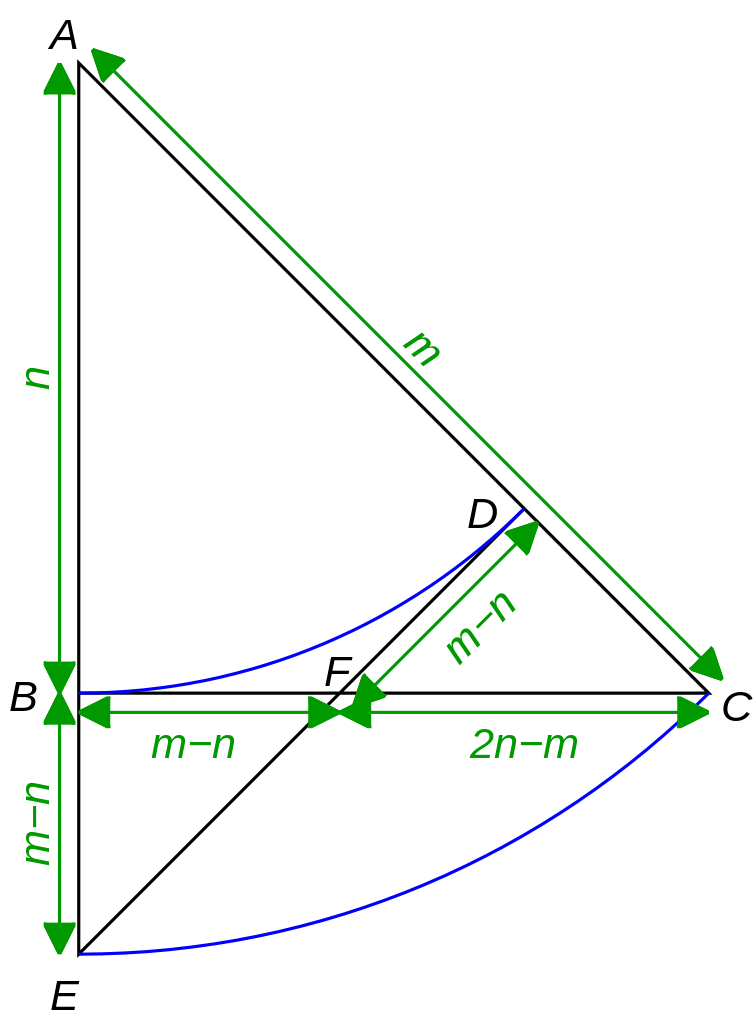
\includegraphics[height=0.25\textwidth]{geometric}
        \caption{A geometric construction.}
        \label{fig:my_label}
    \end{figure}
    }


    \visible<5->{This leads to the constradiction that $(2n-m):(m-n)=m:n$\,.}
    
\end{frame}

\end{document}
